\subsection{Integration der Designvorlagen}
\label{Kommandozeilenprogramme}
Wie bereits in Kapitel \ref{Der FreeDesign-Editor} beschrieben, können die Kunden aus einer Vielzahl Designvorlagen eine Vorlage zur weiteren Gestaltung wählen. 
Diese Vorlagen werden von der hausinternen Grafikabteilung mit dem Programm \emph{Adobe Illustrator}, was eine Software zur Erstellung von Vektor-Grafiken ist \autocite[vgl.][]{Adobe:Illustrator}, erstellt und im SVG-Dateiformat gespeichert. Anschließend werden die SVG-Dateien durch einen Import-Prozess in das Easyprint-Shop-System importiert. Das FreeDesign-Projekt unterstützt diesen Prozess durch die Bereitstellung eines Kommandozeilenprogramms zur automatischen Konvertierung der SVG-Dateien, in ein Dateiformat welches durch den FreeDesign-Editor gelesen werden kann. Die Designvorlagen werden nach der Konvertierung dem Prozess im XML-Format zur weiteren Verarbeitung bereitgestellt. 
Das Programm wird als \emph{draftImporterCli} bezeichnet und dessen Abhängigkeiten werden durch Abbildung \ref{fig:DesignImport} dargestellt.
Die gestrichelten Pfeile stellen die Nutzung von Schnittstellendefinitionen dar und die durchgängigen Pfeile funktionale Abhängigkeiten. Es wird durch \lstinline|draftImporterCli.ts| auf den Ordner \lstinline|stores| zugegriffen, da das Kommandozeilenprogramm Redux nicht nutzt, ist dieser Zugriff ungünstig.


\begin{figure}[H]
    \centering
    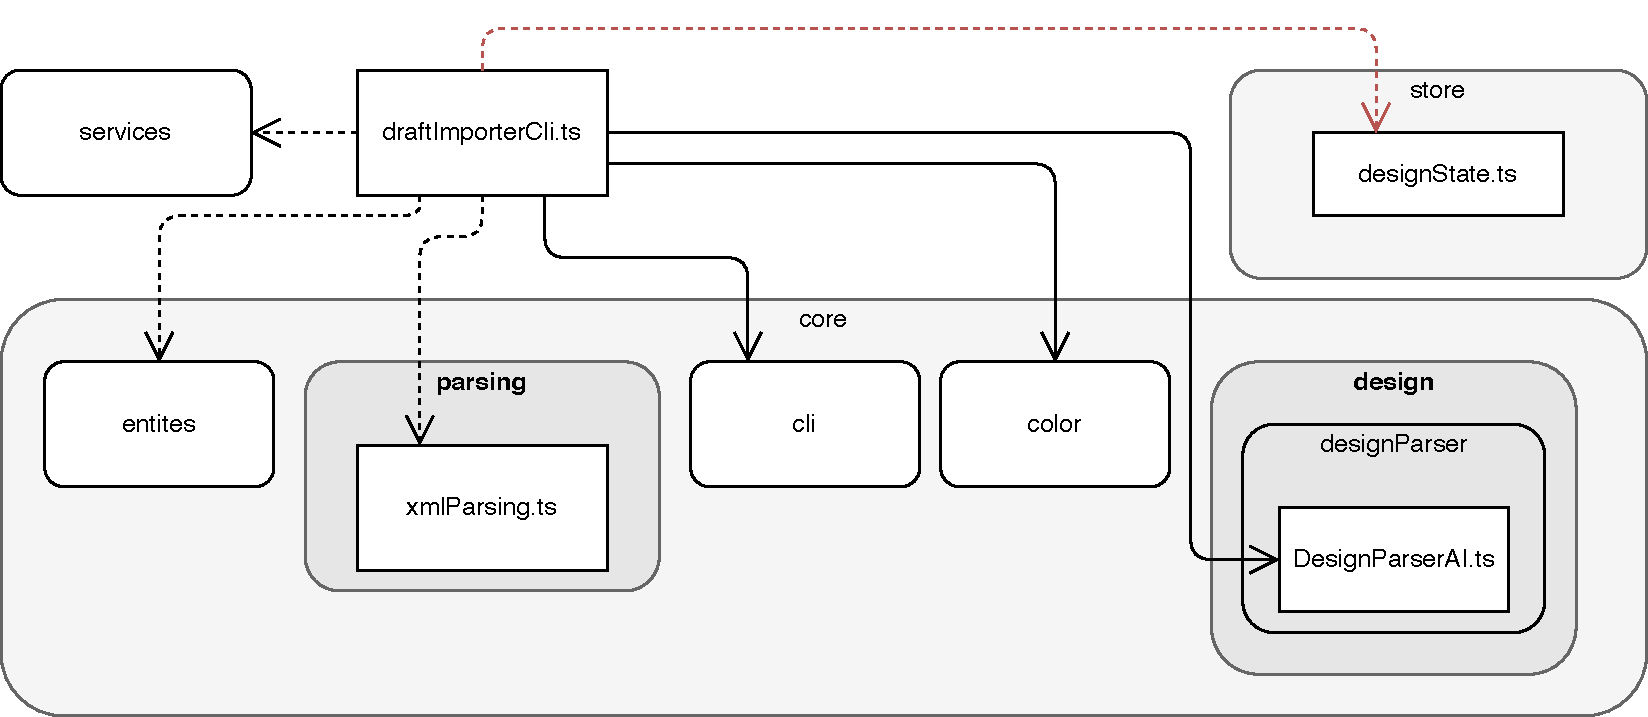
\includegraphics[width=.9\textwidth]{diagrams/Ist-Architektur/draftImporter-analysis.pdf}
    \caption{Abhängigkeiten des Kommandozeilenprogramms \emph{draftImporterCli}}.
    \label{fig:DesignImport}
\end{figure}

In weiteren Schritten des Integrationsprozess werden die Designvorlagen weiterverarbeitet und die \emph{Farb/Sprach-Derivate} erzeugt, die im Abschnitt \ref{sect:Designvorlagen} beschrieben wurden. In in einem finalen Schritt werden die 3D-Vorschaubilder der Designderivate für die Übersichtseite (Abbildung \ref{fig:Designuebersichtseite}) erzeugt. Dieser Schritt benötigt die Designderivate der einzelnen Produktseiten im SVG-Format. Hierfür stellt das FreeDesign-Projekt das Kommandozeilenprogramm \emph{designToSvgCLI} bereit, welches ein Designderivate einließt, welches dem Programm als Argument übergeben wurde. Das Programm konvertiert die einzelnen Designseiten in das SVG-Format und speichert sie als SVG-Dateien in einem Zielordner, welches ebenfalls dem Programm als Argument übergeben wird. 
Die Abhängigkeiten des Kommandozeilenprogramm werden durch Abbildung \ref{fig:DesignToSvg} dargestellt.

\begin{figure}[H]
    \centering
    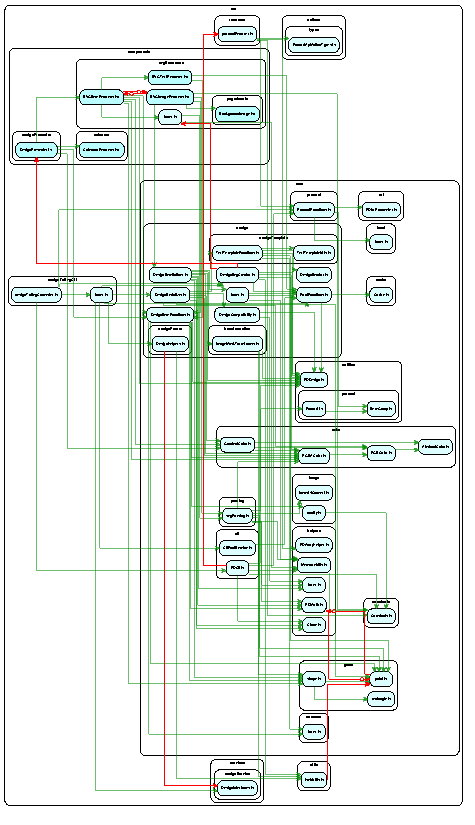
\includegraphics[width=.9\textwidth]{diagrams/Ist-Architektur/designToSvgCLI-analysis.pdf}
    \caption{Abhängigkeiten des Kommandozeilenprogramms \emph{designToSvgCLI}}.
    \label{fig:DesignToSvg}
\end{figure}

